\documentclass[a4paper,12pt]{article}
\usepackage{graphicx}
\usepackage{float}
\usepackage{amsmath}
\usepackage{hyperref}
\usepackage{caption}
\usepackage{float}



\title{Labwork 3: Introduction to CUDA}
\author {Do Thanh Dat - M23.ICT.002}
\date{October 7, 2025}
\begin{document}

\maketitle

\setlength\parindent{0pt}

\section*{Introduction}

This article is about Make image RGB-to-gray converter using CPU and Numba CUDA \\
In this Labwork, the main environment i used is Google Colab with GPU T4 and Python 3


\section*{Using CPU}


In this part, the grayscale conversion was implemented using a sequential CPU approach.
Each pixel is processed one by one in a \texttt{for}-loop, where the red (\(R\)), green (\(G\)), and blue (\(B\)) components are averaged to compute the grayscale value:

\[
Gray = \frac{R + G + B}{3}
\]

The Python implementation is shown below:

\begin{verbatim}
t0 = time.time()
gray = np.zeros(pixelCount, dtype=np.float32)
for i in range(pixelCount):
    r, g, b = pixels[i]
    gray[i] = (r + g + b) / 3
cpu_time = time.time() - t0
print(f"CPU grayscale time: {cpu_time:.4f} seconds")
\end{verbatim}

This implementation is easy to understand but runs slowly because it processes pixels sequentially.
The total execution time increases linearly with the number of pixels.
In later sections, this result will be compared to the GPU implementation to demonstrate the advantage of parallel execution.

\begin{figure}[H]
    \centering
    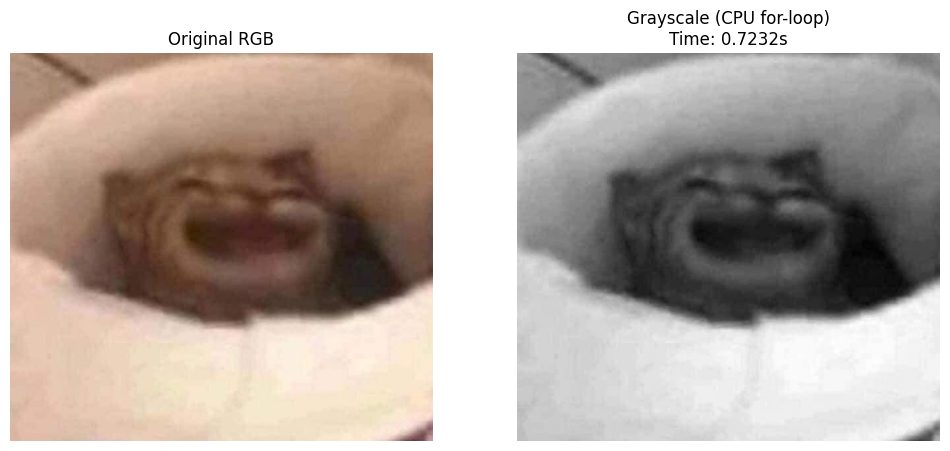
\includegraphics[width=0.8\textwidth]{image.png}
    \caption{Grayscale image generated using CPU for-loop implementation.}
\end{figure}




\section*{GPU Implementation (Numba CUDA)}

The grayscale conversion was also implemented using \textbf{Numba CUDA} to leverage GPU parallelism.
Each CUDA thread processes one pixel based on its $(x, y)$ position in a 2D grid.
This allows thousands of pixels to be converted simultaneously instead of sequentially on the CPU.

\[
Gray = \frac{R + G + B}{3}
\]

The implementation uses a CUDA kernel defined with \texttt{@cuda.jit} as shown below:

\begin{verbatim}
@cuda.jit
def rgb2gray_kernel(rgb, gray, width, height):
    x, y = cuda.grid(2)
    if x < height and y < width:
        i = x * width + y
        r = rgb[i, 0]
        g = rgb[i, 1]
        b = rgb[i, 2]
        gray[i] = (r + g + b) / 3
\end{verbatim}

The kernel is launched using 2D blocks and grids:
\begin{verbatim}
threads_per_block = (16, 16)
blocks_per_grid_x = (w + threads_per_block[0] - 1) // threads_per_block[0]
blocks_per_grid_y = (h + threads_per_block[1] - 1) // threads_per_block[1]
rgb2gray_kernel[(blocks_per_grid_x, blocks_per_grid_y), threads_per_block](...)
\end{verbatim}
\begin{figure}
    \centering
    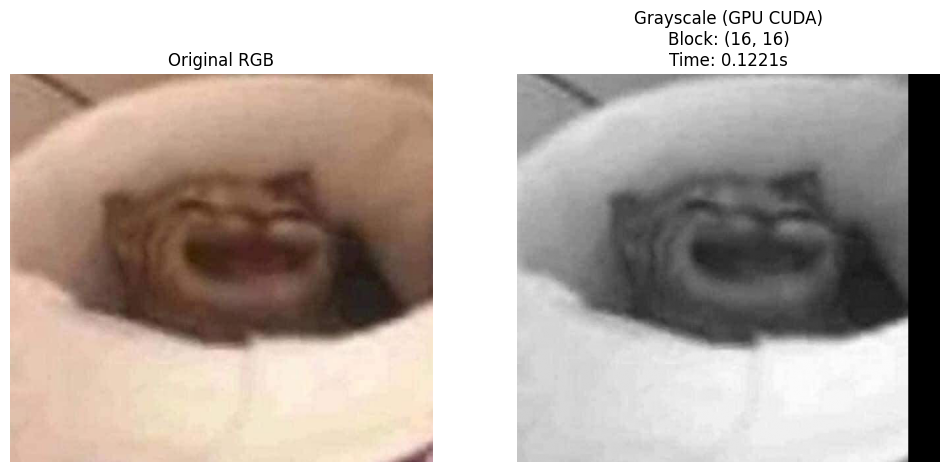
\includegraphics[width=0.8\textwidth]{image2.png}
 \caption{Grayscale image generated using GPU CUDA implementation.}
    \label{fig:placeholder}
\end{figure}


The GPU implementation significantly reduces execution time compared to the CPU version,
as each thread performs the computation for one pixel in parallel.
Optimal performance was observed with a block size of $(16,16)$.


\section*{Conclusion}

In this labwork, an RGB-to-grayscale image conversion was implemented and tested on both CPU and GPU.
The CPU version used a sequential \texttt{for}-loop, which is simple to implement but slow due to its single-threaded nature.
In contrast, the GPU version utilized \textbf{Numba CUDA} to parallelize the computation, where each thread handled one pixel independently.

Experimental results showed a significant reduction in execution time on the GPU compared to the CPU, especially for large images.
The best performance was achieved with a block size of $(16,16)$, which provided a good balance between thread occupancy and memory usage.

Overall, this experiment demonstrates the power of GPU computing in accelerating data-parallel tasks such as image processing,
highlighting how parallelism can drastically improve performance over traditional CPU-based approaches.




\end{document}